% Options for packages loaded elsewhere
\PassOptionsToPackage{unicode}{hyperref}
\PassOptionsToPackage{hyphens}{url}
\PassOptionsToPackage{dvipsnames,svgnames,x11names}{xcolor}
%
\documentclass[
  english,
  a4paper,
]{article}
\usepackage{amsmath,amssymb}
\usepackage{lmodern}
\usepackage{iftex}
\ifPDFTeX
  \usepackage[T1]{fontenc}
  \usepackage[utf8]{inputenc}
  \usepackage{textcomp} % provide euro and other symbols
\else % if luatex or xetex
  \usepackage{unicode-math}
  \defaultfontfeatures{Scale=MatchLowercase}
  \defaultfontfeatures[\rmfamily]{Ligatures=TeX,Scale=1}
\fi
% Use upquote if available, for straight quotes in verbatim environments
\IfFileExists{upquote.sty}{\usepackage{upquote}}{}
\IfFileExists{microtype.sty}{% use microtype if available
  \usepackage[]{microtype}
  \UseMicrotypeSet[protrusion]{basicmath} % disable protrusion for tt fonts
}{}
\makeatletter
\@ifundefined{KOMAClassName}{% if non-KOMA class
  \IfFileExists{parskip.sty}{%
    \usepackage{parskip}
  }{% else
    \setlength{\parindent}{0pt}
    \setlength{\parskip}{6pt plus 2pt minus 1pt}}
}{% if KOMA class
  \KOMAoptions{parskip=half}}
\makeatother
\usepackage{xcolor}
\IfFileExists{xurl.sty}{\usepackage{xurl}}{} % add URL line breaks if available
\IfFileExists{bookmark.sty}{\usepackage{bookmark}}{\usepackage{hyperref}}
\hypersetup{
  pdftitle={TODO title},
  pdflang={en},
  colorlinks=true,
  linkcolor={blue},
  filecolor={Maroon},
  citecolor={blue},
  urlcolor={blue},
  pdfcreator={LaTeX via pandoc}}
\urlstyle{same} % disable monospaced font for URLs
\usepackage[margin=25mm]{geometry}
\usepackage{longtable,booktabs,array}
\usepackage{calc} % for calculating minipage widths
% Correct order of tables after \paragraph or \subparagraph
\usepackage{etoolbox}
\makeatletter
\patchcmd\longtable{\par}{\if@noskipsec\mbox{}\fi\par}{}{}
\makeatother
% Allow footnotes in longtable head/foot
\usepackage{footnote} % For some unknown reason, footnotehyper clashes with French
\makesavenoteenv{longtable}
\usepackage{graphicx}
\makeatletter
\def\maxwidth{\ifdim\Gin@nat@width>\linewidth\linewidth\else\Gin@nat@width\fi}
\def\maxheight{\ifdim\Gin@nat@height>\textheight\textheight\else\Gin@nat@height\fi}
\makeatother
% Scale images if necessary, so that they will not overflow the page
% margins by default, and it is still possible to overwrite the defaults
% using explicit options in \includegraphics[width, height, ...]{}
\setkeys{Gin}{width=\maxwidth,height=\maxheight,keepaspectratio}
% Set default figure placement to htbp
\makeatletter
\def\fps@figure{htbp}
\makeatother
\setlength{\emergencystretch}{3em} % prevent overfull lines
\providecommand{\tightlist}{%
  \setlength{\itemsep}{0pt}\setlength{\parskip}{0pt}}
\setcounter{secnumdepth}{5}
\newlength{\cslhangindent}
\setlength{\cslhangindent}{1.5em}
\newlength{\csllabelwidth}
\setlength{\csllabelwidth}{3em}
\newlength{\cslentryspacingunit} % times entry-spacing
\setlength{\cslentryspacingunit}{\parskip}
\newenvironment{CSLReferences}[2] % #1 hanging-ident, #2 entry spacing
 {% dont indent paragraphs
  \setlength{\parindent}{0pt}
  % turn on hanging indent if param 1 is 1
  \ifodd #1
  \let\oldpar\par
  \def\par{\hangindent=\cslhangindent\oldpar}
  \fi
  % set entry spacing
  \setlength{\parskip}{#2\cslentryspacingunit}
 }%
 {}
\usepackage{calc}
\newcommand{\CSLBlock}[1]{#1\hfill\break}
\newcommand{\CSLLeftMargin}[1]{\parbox[t]{\csllabelwidth}{#1}}
\newcommand{\CSLRightInline}[1]{\parbox[t]{\linewidth - \csllabelwidth}{#1}\break}
\newcommand{\CSLIndent}[1]{\hspace{\cslhangindent}#1}

%%%%%%%% START HEADER PARTIAL %%%%%%%%%%%%

% Formatting of tables & knitr::kable and kableExtra functionality
\usepackage{float}
\usepackage{colortbl}
\usepackage{pdflscape}
\usepackage{tabu}
\usepackage{threeparttable}

% Line numbering

% endfloat stuff

% fancyhdr pagestyle

% Environment for keywords
\makeatletter
\newcommand\keywordsname{Keywords}
\newenvironment*{keywords}[1][\keywordsname]{\if@twocolumn \else \small \quotation \fi \begin{center} \textbf{\textit{#1} \\}}{\end{center}\if@twocolumn \else \small \endquotation \fi}
\newenvironment*{keywordsinline}[1][\keywordsname]{\if@twocolumn \else \small \quotation \fi \begin{center} \textbf{\textit{#1}: }}{\end{center}\if@twocolumn \else \small \endquotation \fi}
\makeatother

% Environment for abstract that takes new abstract name
\newenvironment{renameableabstract}[1][\abstractname]{\let\oldabstractname\abstractname \renewcommand{\abstractname}{#1} \begin{abstract}}{\end{abstract} \renewcommand{\abstractname}{\oldabstractname}}

%%%%%%%% END HEADER PARTIAL %%%%%%%%%%%%

\usepackage{booktabs}
\usepackage{longtable}
\usepackage{array}
\usepackage{multirow}
\usepackage{wrapfig}
\usepackage{float}
\usepackage{colortbl}
\usepackage{pdflscape}
\usepackage{tabu}
\usepackage{threeparttable}
\usepackage{threeparttablex}
\usepackage[normalem]{ulem}
\usepackage{makecell}
\usepackage{xcolor}
\ifXeTeX
  % Load polyglossia as late as possible: uses bidi with RTL langages (e.g. Hebrew, Arabic)
  \usepackage{polyglossia}
  \setmainlanguage[]{}
\else
  \usepackage[english,main=english]{babel}
% get rid of language-specific shorthands (see #6817):
\let\LanguageShortHands\languageshorthands
\def\languageshorthands#1{}
\fi
\ifLuaTeX
  \usepackage{selnolig}  % disable illegal ligatures
\fi

\title{TODO title}

%%%%%%% START AUTHOR PARTIAL %%%%%%%%%%%%%%%

%%%%% Authors, affiliations and author notes stuff %%%%%

% Macros for creating and referencing stored reference
\makeatletter
\def\MyNewLabel#1#2#3{\expandafter\gdef\csname #1@#2\endcsname{#3}}

\def\MyRef#1#2{\@ifundefined{#1@#2}{???}{\csname #1@#2\endcsname}}

\newcommand*\ifcounter[1]{%
  \ifcsname c@#1\endcsname
    \expandafter\@firstoftwo
  \else
    \expandafter\@secondoftwo
  \fi
}
\makeatother

% Create labels for Addresses if the are given by code
\MyNewLabel{ADDRTXT}{Stanford}{Stanford University}

% Create labels for Footnotes if they are given by code
\MyNewLabel{ANOTETXT}{corresp}{Corresponding author. Email: \href{mailto:vboyce@stanford.edu}{\nolinkurl{vboyce@stanford.edu}}}

%%% Special footnotes for addresses and author footnotes
\usepackage{bigfoot}
\DeclareNewFootnote{Addr}[arabic] % Only used for NOT authblk
\DeclareNewFootnote{ANote}[fnsymbol]

%%% Address and author notes as a function of format %%%
 % Use authblk for affiliations %%%%%%%%%%%
\usepackage{authblk}

% Always separate by commas
\renewcommand\Authsep{, }
\renewcommand\Authand{, }
\renewcommand\Authands{, }

% Counter for addresses and footnotes
\newcounter{addrcnt}

% thanks definition that doesnt produce superscript marks
\makeatletter
\newcommand*\createaddrlblbycode[1]{%
  \ifcounter{ADDRLBL@#1}
    {}
    {\refstepcounter{addrcnt}\newcounter{ADDRLBL@#1}\setcounter{ADDRLBL@#1}{\value{addrcnt}}}%
}

\newcommand*\addrlblbycode[1]{\arabic{ADDRLBL@#1}}

\newcommand*\addrbycode[1]{%
  \ifcounter{ADDR@#1}
    {}
    {\newcounter{ADDR@#1}%
     \affil[\addrlblbycode{#1}]{\MyRef{ADDRTXT}{#1}}}%
}

\newcommand*\createanotelblbycode[1]{%
  \ifcounter{ANOTELBL@#1}
    {}
    {\refstepcounter{footnoteANote}\newcounter{ANOTELBL@#1}\setcounter{ANOTELBL@#1}{\value{footnoteANote}}}%
}

\newcommand*\anotelblbycode[1]{\fnsymbol{ANOTELBL@#1}}

\newcommand*\anotebycode[1]{%
  \ifcounter{ANOTE@#1}
    {}
    {\newcounter{ANOTE@#1}%
     \footnotetextANote[\value{ANOTELBL@#1}]{\MyRef{ANOTETXT}{#1}}}%
}
\makeatother


\createaddrlblbycode{Stanford}


\createanotelblbycode{corresp}

\author[%
\addrlblbycode{Stanford}%
,%
$\anotelblbycode{corresp}$%
]{Veronica Boyce}

\addrbycode{Stanford}


\createaddrlblbycode{Stanford}



\author[%
\addrlblbycode{Stanford}%
]{Robert Hawkins}

\addrbycode{Stanford}


\createaddrlblbycode{Stanford}



\author[%
\addrlblbycode{Stanford}%
]{Noah D. Goodman}

\addrbycode{Stanford}


\createaddrlblbycode{Stanford}



\author[%
\addrlblbycode{Stanford}%
]{Michael C. Frank}

\addrbycode{Stanford}


%endif(authblk)

%%%%%%%%% END AUTHOR PARTIAL %%%%%%%%

\date{}

\begin{document}
\maketitle

%%%%%%%%%% START AFTER TITLE PARTIAL %%%%%%%%%%%%%
\anotebycode{corresp}


%%%%%%%%%% END AFTER TITLE PARTIAL %%%%%%%%%%%%%


\begin{otherlanguage}{english}

\begin{abstract}
\emph{This is an abstract in italics.}

This is the second paragraph not in italics.

\end{abstract}

\end{otherlanguage}

\begin{otherlanguage}{english}

\begin{keywords}
One keyword; Yet another keyword

\end{keywords}

\end{otherlanguage}

\hypertarget{introduction}{%
\section{Introduction}\label{introduction}}

Verbal communication is an integral part of our daily lives. We coordinate schedules with partners, socialize with friends over board games, learn and teach in seminar classes, and listen to podcasts. Communicative environments range in size from one-on-one dialogue to broadcast communication to large groups, but the goal of efficient communication is shared across these (\protect\hyperlink{ref-traum2004}{Traum 2004}, \protect\hyperlink{ref-branigan2006}{\textbf{branigan2006?}}, \protect\hyperlink{ref-ginzburg2005}{\textbf{ginzburg2005?}}). Shared referring expressions are a necessity for efficient communication; a thing or an idea needs some sort of name that the interlocutors will jointly understand. In many cases, there are widely shared conventionalized expressions for objects or ideas, but in other cases, spontaneous ad-hoc expressions must be invented.

The formation of these new reference expressions is well-studied in dyadic contexts and has been a case study for efficient communication more broadly. But these dynamics may be different in larger groups, which are less studied. Our current work builds on the dyadic reference game tradition by extending it to larger groups.

Clark \& Wilkes-Gibbs (\protect\hyperlink{ref-clarkReferringCollaborativeProcess1986}{1986}) established an experimental method for studying the emergence of new referring expressions that has now become standard (building on \protect\hyperlink{ref-kraussChangesReferencePhrases1964}{Krauss \& Weinheimer 1964}, \protect\hyperlink{ref-kraussConcurrentFeedbackConfirmation1966}{\textbf{kraussConcurrentFeedbackConfirmation1966?}}). Two participants see the same set of tangram figures; the speaker describes each figure in turn so the listener can select the target from the set of figures. The speaker and listener repeat this process with the same images over a series of blocks. Early descriptions are long and make reference to multiple features in the figure, but in later iterations, shorthand conventional names for each figure emerge; this shortening of utterances is called `reduction'.

Recently, online participant recruitment and web-based experiments have made it possible to study this convergence in larger populations (\protect\hyperlink{ref-haber2019}{Haber et al. 2019}, \protect\hyperlink{ref-hawkinsCharacterizingDynamicsLearning2020}{Hawkins et al. 2020}). In Hawkins et al. (\protect\hyperlink{ref-hawkinsCharacterizingDynamicsLearning2020}{2020}), 83 pairs completed a similar iterated reference experiment where they communicated via a chat box. Speakers reduced their utterances, producing fewer words per image in later blocks than in earlier blocks, in line with results from face-to-face, oral paradigms.\footnote{We use ``speaker'' and ``listener'' to refer to the roles describing and selecting targets, regardless of communication modality.}

How does this process proceed in multi-party communication? In a dyad, speakers can tailor their utterances to the one listener, but in large groups, speakers must balance the competing needs of different listeners (\protect\hyperlink{ref-schober1989}{Schober \& Clark 1989}, \protect\hyperlink{ref-tolins2016}{Tolins \& Fox Tree 2016}). These effects likely vary by both the knowledge state of and communication channels available to the listeners (\protect\hyperlink{ref-fox-tree2013}{\textbf{fox-tree2013?}}, \protect\hyperlink{ref-horton2002}{\textbf{horton2002?}}, \protect\hyperlink{ref-horton2005}{\textbf{horton2005?}}). Prior work has focused on manipulating knowledge states by adding new listeners to established groups.

\begin{figure*}[t!]

{\centering 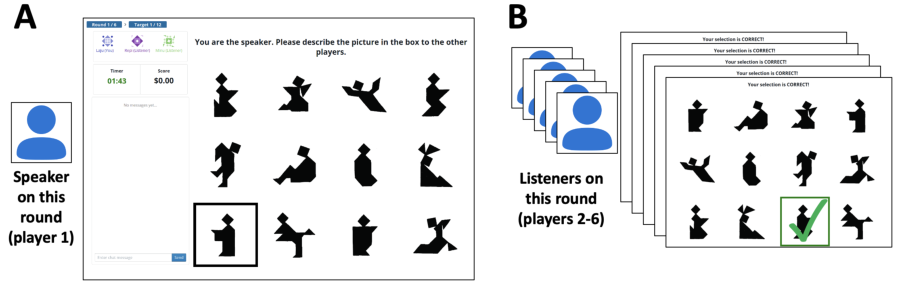
\includegraphics[width=1\linewidth]{figs/interface-1} 

}

\caption{All participants saw all 12 tangram images. (A) Speaker's view during selection phase. (B) During the feedback stage, speakers saw what figure each person chose, but listeners only learned if their selection was correct or incorrect. Listeners were not shown what other listeners chose. \label{game}}\label{fig:interface}
\end{figure*}

In this context, one approach for speakers is to `aim low' and produce utterances tailored to the least knowledgeable listener (\protect\hyperlink{ref-yoonAimLowMechanisms2018a}{\textbf{yoonAimLowMechanisms2018a?}}). For instance, in Yoon \& Brown-Schmidt (\protect\hyperlink{ref-yoonAdjustingConceptualPacts2014}{2014}), speakers developed conventions with one listener but then used longer descriptions with a new listener. Another strategy for speakers is to integrate across listeners and balance efficiency with informativeness by `aiming in the middle'. In Yoon \& Brown‐Schmidt (\protect\hyperlink{ref-yoonAudienceDesignMultiparty2019}{2019}), speakers communicating to a mixed group of 3 experienced listeners and 1 naive listener used shorter utterances and made fewer accommodations than they did in groups with a greater fraction of naive listeners. Both of these strategies predict that larger groups will be slower to converge than smaller groups.

Disagreements about how to conceptualize referents can also slow groups down. In (\protect\hyperlink{ref-weberCulturalConflictMerger2003}{\textbf{weberCulturalConflictMerger2003?}}), pairs of participants played a reference game with the same image sets before a listener switched groups and joined a different pair, making a group of three. The addition of the new listener slowed both listeners down for multiple rounds. When a listener switched groups, they brought preconceptions about how the pictures should be described which conflicted with how the speaker was used to describing the images. This result predicts that, with more perspectives in play, larger groups may have more difficulty agreeing on common conceptualizations.

In general, listeners expect speakers to maintain conventions and stick to descriptions that were similar to successful descriptions. However, listeners were not surprised to hear different descriptions of a familiar object if it came from a new speaker who had just entered the room (\protect\hyperlink{ref-metzingWhenConceptualPacts2003}{Metzing \& Brennan 2003}). It's unclear what this finding predicts about new speakers who are present as fellow listeners during prior blocks -- will listeners expect them to maintain conventions?

Work on multi-party communication has focused on the addition of a new person into a pair or group that had built up some shared representations. Our present work complements this prior work by examining the effect of group size during the process of convention formation. We extend the dyadic repeated reference game paradigm of Hawkins et al. (\protect\hyperlink{ref-hawkinsCharacterizingDynamicsLearning2020}{2020}) to games for 2--6 players who rotate between speaker and listener roles. This paradigm allows us to confirm that these findings in dyads extend to larger groups: that accuracy and speed will increase across blocks (question 1) and that speakers will reduce their utterances (produce fewer words) in later blocks (question 2). Additionally, we will be able to test for trends across group size, allowing us to ask whether smaller groups use shorter utterances and reduce faster than larger groups (question 3) and how conventions emerge in larger groups (question 4). In sum, these analyses will fill a gap in the literature by providing a basic characterization of how convention-formation and communication occurs in larger groups.

\hypertarget{experiment-1}{%
\section{Experiment 1}\label{experiment-1}}

\hypertarget{methods}{%
\subsection{Methods}\label{methods}}

Building on the methods of Hawkins et al. (\protect\hyperlink{ref-hawkinsCharacterizingDynamicsLearning2020}{2020}), we used Empirica (\protect\hyperlink{ref-almaatouqEmpiricaVirtualLab2020}{Almaatouq et al. 2020}) to create real-time multi-player reference games. In each game, one of the players started as the speaker who saw an array of tangrams with one highlighted (Figure \ref{game}A) and communicated which figure to click to the other players (listeners). After the speaker had identified each of the 12 images in turn, the speaker role rotated to another player and the process repeated with the same images. In total, there were 6 blocks, giving each player at least one chance to be the speaker. We recorded what participants said in the chat, as well as who selected what image and how long they took to make their selections.\footnote{Code to run the experiment, as well as data and analysis code are available at \url{https://osf.io/qdvbr/?view_only=47aebfde243f405e9c42a45cacb697d2}.} We report how we determined our sample size, all data exclusions, all manipulations, and all measures in the study.\footnote{Our preregistrations are at \url{https://osf.io/cn9f4/?view_only=7fdacd698b24465cb1a8699050af5bfc} and \url{https://osf.io/rpz67?view_only=5284203e2b644fc5ac39cf3e723b9a7e}.}

\hypertarget{participants}{%
\subsubsection{Participants}\label{participants}}

We recruited participants between May and July 2021 using the Prolific platform; participants had all self-reported as fluent native English speakers on Prolific's demographic prescreen. Participants were paid \$7 for 2-player games, \$8.50 for 3-player games, \$10 for 4-player games, and \$11 for 5- and 6-player games (with the intention of a \$10 hourly rate), in addition to up to \$2.88 in performance bonuses. A total of 390 people each participated in one game.

\hypertarget{materials}{%
\subsubsection{Materials}\label{materials}}

We used the 12 tangram images used by Hawkins et al. (\protect\hyperlink{ref-hawkinsCharacterizingDynamicsLearning2020}{2020}) and Clark \& Wilkes-Gibbs (\protect\hyperlink{ref-clarkReferringCollaborativeProcess1986}{1986}) (see Figure \ref{game}). These images were displayed in a grid with order randomized for each participant (thus descriptions such as ``top left'' were ineffective as the image might be in a different place on the speaker's and listeners' screens). The same images were used every block.

\hypertarget{procedure}{%
\subsubsection{Procedure}\label{procedure}}

\begin{table}[h]
\centering
\begin{tabular}{ccc}
  \hline
Players & Partial & Complete \\ 
  \hline
  2 &   4 &  15 \\ 
    3 &   2 &  18 \\ 
    4 &   2 &  19 \\ 
    5 &   3 &  17 \\ 
    6 &   6 &  12 \\ 
   \hline
\end{tabular}
\caption{Number of games run for each player count.\label{parts}} 
\end{table}

We implemented the experiment using Empirica, a Javascript-based platform for running real-time interactive experiments online (\protect\hyperlink{ref-almaatouqEmpiricaVirtualLab2020}{Almaatouq et al. 2020}). From Prolific, participants were directed to our website where they navigated through a self-paced series of instruction pages explaining the game. Participants had to pass a quiz to be able to play the game. They were then directed to a ``waiting room'' screen until their partners were ready.

Once the game started, participants saw screens like Figure \ref{game}A. Each trial, the speaker described the highlighted tangram image so that the listeners could identify and click it. All participants were free to use the chat box to communicate, but listeners could only click once the speaker had sent a message. Once a listener clicked, they could not change their selection. There was no signal to the speaker or other listeners about who had already made a selection.

Once all listeners had selected (or a 3-minute timer ran out), participants were given feedback (Figure \ref{game}B). Listeners learned whether they individually had chosen correctly or not; listeners who were incorrect were not told the correct answer. The speaker saw which tangram each listener had selected, but listeners did not. This feedback regime is different from Hawkins et al. (\protect\hyperlink{ref-hawkinsCharacterizingDynamicsLearning2020}{2020}) where listeners were shown what the right answer was during feedback. We made this change to prevent listeners from learning conventions purely as a memorized mapping between utterance and correct answer.

Listeners got 4 points for each correct answer; the speaker got points equal to the average of the listeners' points. These points translated into performance bonus at the end of the experiment.

In each block, each of the 12 tangrams was indicated to the speaker once. The same person was the speaker for an entire block, but participants rotated roles between blocks. Thus, over the course of the 6 blocks, participants were speakers 3 times in 2-player games, twice in 3-player games, once or twice in 4 and 5-player games, and once in 6-player games. Rotating the speaker was chosen to keep participants more equally engaged (the speaker role is more work), and to give a more robust test for reduction and convention.

After the game finished, participants were given a survey asking for optional demographic information and feedback on their experience with the game.

\hypertarget{data-pre-processing-and-exclusions}{%
\subsubsection{Data pre-processing and exclusions}\label{data-pre-processing-and-exclusions}}

Participants could use the chat box freely, which meant that the chat transcript contained some non-referential language. The first author skimmed through the chat transcripts, tagging utterances that did not refer to the current tangram. These were primarily pleasantries (``Hello''), meta-commentary about how well or fast the task was going, and confirmations or denials (``ok'', ``got it'', ``yes'', ``no''). We exclude these utterances from our analyses. Note that chat lines sometimes included non-referential words in addition to words referring to the tangrams (``ok, so it looks like a zombie'', ``yes, the one with legs''); these lines were retained intact.

Our intended sample size was 20 complete games in each group size, but we ended up with fewer due to games not filling or participants disconnecting early (Table \ref{parts}). We excluded incomplete blocks from analyses, but included complete blocks from partial games.

\hypertarget{results}{%
\subsection{Results}\label{results}}

\hypertarget{accuracy-and-speed}{%
\subsubsection{Accuracy and Speed}\label{accuracy-and-speed}}

Our first question was whether accuracy and speed increased across groups of different sizes.

\hypertarget{accuracy-is-high-and-increasing.}{%
\paragraph{Accuracy is high and increasing.}\label{accuracy-is-high-and-increasing.}}

\begin{figure}[t]

{\centering \includegraphics[width=1\linewidth]{figs/accuracy-1} 

}

\caption{Players' accuracy at correctly selecting the target figure by block and group size. Accuracy increases across blocks. \label{accuracy}}\label{fig:accuracy}
\end{figure}

Most individuals were accurate in their selections, with accuracy rising across blocks (Figure \ref{accuracy}). In a logistic model of accuracy\footnote{correct.num\(\sim\) block \(\times\) numPlayers This and all subsequent regression models were run in brms with weakly regularizing priors.}, participants are more accurate in later blocks (block: Est=0.38, CrI={[}0.25, 0.5{]}), and there was no strong effect of group size on accuracy (numPlayers: Est=-0.02, CrI={[}-0.08, 0.03{]}) or interaction between block and group size (block:numPlayers: Est=-0.01, CrI={[}-0.04, 0.01{]}).

\hypertarget{participants-speed-up-in-later-blocks.}{%
\paragraph{Participants speed up in later blocks.}\label{participants-speed-up-in-later-blocks.}}

\begin{figure}[t]

{\centering \includegraphics[width=1\linewidth]{figs/time-1} 

}

\caption{How long listeners took to select a figure in seconds by block and group size. Listeners selected images faster in later blocks. Only times for correct responses are shown.\label{time}}\label{fig:time}
\end{figure}

Participants selected images faster in later blocks (Figure \ref{time}), although there was wide variability. In a linear model of selection time\footnote{time\(\sim\) block \(\times\) numPlayers}, participants got faster across blocks (block: Est=-10.03, CrI={[}-11.03, -9.03{]}) and were slightly slower in larger games (numPlayers: Est=1.03, CrI={[}0.4, 1.66{]}). This speed up is consistent with prior work by (\protect\hyperlink{ref-weberCulturalConflictMerger2003}{\textbf{weberCulturalConflictMerger2003?}}) which used speed as the dependent measure. Wide variability in selection time meant that especially for larger groups, there was a wide spread in how long it took groups to complete the experiment.

\hypertarget{reduction}{%
\subsubsection{Reduction}\label{reduction}}

Our second question was whether speakers reduce their referring expressions in larger groups.

\hypertarget{speakers-utterances-reduce-in-length.}{%
\paragraph{Speakers' utterances reduce in length.}\label{speakers-utterances-reduce-in-length.}}

\begin{figure}[h]

{\centering \includegraphics[width=1\linewidth]{figs/variability-1} 

}

\caption{Number of words from speaker (total, across all 12 figures) in a block. Each colored line is one group, the overall trend is shown in black. Across group size, the number of words decreases as conventions emerge, but convention formation is not a smooth process, and there is variability between speakers.\label{variability}}\label{fig:variability}
\end{figure}

As shown in Figure \ref{variability}, the number of words produced by speakers decreases over the course of rounds, both in aggregate and for many individual groups. Nonetheless, in some groups, a later speaker may be more verbose than an earlier speaker. Speakers make longer utterances in early blocks that reduce to shorter utterances in later blocks. From a linear model\footnote{words\(\sim\) block \(\times\) numPlayers~+ (block\textbar tangram)~+ (1\textbar playerId)~+ (1\textbar tangram\_group)~+ (block\textbar gameId)}, the effect of being one block later is -3.35 (CrI={[}-4.58, -2.13{]}) words.

\hypertarget{listeners-rarely-talk.}{%
\paragraph{Listeners rarely talk.}\label{listeners-rarely-talk.}}

Listeners often don't talk much, but are more likely to ask questions or make clarification in early blocks. In a linear regression for the number of words each listener said \footnote{words\(\sim\) block \(\times\) numPlayers~+ (block\textbar tangram)~+ (1\textbar playerId)~+ (1\textbar tangram\_group)~+ (block\textbar gameId)}, there was an effect of block (block: Est=-0.48, CrI={[}-0.79, -0.18{]}), but no clear effect of game size (numPlayers: Est=0.2, CrI={[}-0.13, 0.51{]}).

\hypertarget{effects-of-group-size-on-conventions}{%
\subsubsection{Effects of group size on conventions}\label{effects-of-group-size-on-conventions}}

Our third question was whether smaller groups would use fewer words or reduce faster than larger groups.

\hypertarget{larger-groups-say-more.}{%
\paragraph{Larger groups say more.}\label{larger-groups-say-more.}}

The overall effect of having more players in a group is 1.67 (CrI={[}0.68, 2.71{]}) words from the speaker per trial per additional player. There is no clear interaction between block and group size (block:numPlayers: Est=-0.1, CrI={[}-0.39, 0.18{]}). Larger groups saying more is consistent with predictions from audience design that with more listeners to accommodate, the speaker may use multiple conceptualizations, either initially as a hedge or in response to listener clarifications.

\hypertarget{speaker-experience-does-not-fully-explain-group-size-effects.}{%
\paragraph{Speaker experience does not fully explain group size effects.}\label{speaker-experience-does-not-fully-explain-group-size-effects.}}

One potential concern is that group size correlates with whether the speaker has had the speaker role before (smaller groups repeat speakers more). To address this confound, we coded for whether the speaker has been speaker in an earlier block\footnote{words\(\sim\) block \(\times\) numPlayers~+ block \(\times\) speaker.repeat~+ (block\textbar tangram)~+ (1\textbar playerId)~+ (1\textbar tangram\_group)~+ (block\textbar gameId)}. Repeat speakers do use fewer words (speaker.repeat: Est=-8.55, CrI={[}-10.41, -6.79{]}), but there are still effects of group size (numPlayers: Est=1.63, CrI={[}0.58, 2.66{]}) and block (block: Est=-5.26, CrI={[}-6.84, -3.69{]}). The effects of block and repeat speaker are subadditive (block:speaker.repeat: Est=3.2, CrI={[}2.65, 3.78{]}), and there is minimal interaction between block and group size (block:numPlayers: Est=0.08, CrI={[}-0.22, 0.41{]}).

\hypertarget{development-of-conventions}{%
\subsubsection{Development of conventions}\label{development-of-conventions}}

Our final question was how conventions emerge in larger groups.

\hypertarget{speakers-who-dont-know-the-convention-reduce-less.}{%
\paragraph{Speakers who don't know the convention reduce less.}\label{speakers-who-dont-know-the-convention-reduce-less.}}

In our games (which had limited feedback), listeners who got a tangram wrong didn't have a way of knowing what the right answer was unless they asked for clarification in the chat. If a speaker got a tangram wrong as a listener in the previous block, they may not have known the conventional description that went with it, and thus were unlikely to follow the convention. If we assume that reduction is a sign of convention development, then speakers should say more words when they got the tangram wrong the previous block. We added prior errors as an additional predictor to our regression predicting number of words and found that speakers said more words for tangrams after they were incorrect (numPlayers: Est=2.18, CrI={[}0.93, 3.44{]}).

\hypertarget{smaller-groups-reduce-and-stabilize-conventions-sooner.}{%
\paragraph{Smaller groups reduce and stabilize conventions sooner.}\label{smaller-groups-reduce-and-stabilize-conventions-sooner.}}

\begin{figure*}[h]

{\centering \includegraphics[width=0.8\linewidth]{figs/similarity-1} 

}

\caption{Comparison of the content words is the final (6th) block to words in previous blocks. (A) The proportion 6th block content words found in each prior block. (B) The proportion 6th block content words that were first used by the speaker in each block. Smaller games have higher overlap and a greater proportion of words originating earlier. \label{similarity}}\label{fig:similarity}
\end{figure*}

Another angle to look at conventions is to take the speaker's utterances in the last block as the ``convention'', and look at how far back they started. We took the contentful words said by the speaker in the last block and looked at how many of them were used to describe that tangram in prior rounds.\footnote{Contentful words were defined as all words in a referential message with a part of speech identified by the Spacy (\url{http://spacy.io}) tagger as being a noun, verb, or adjective; that were not on the Spacy stop word list; and that did not have a lemma in the set {[}`look',`like',`body',`person',`man',`guy'{]}, a list generated as being extremely common vocabulary across tangrams.} Then we calculated the proportion overlap between the last block utterance and earlier blocks, shown in Figure \ref{similarity}A. In a linear model of the overlap between an earlier block and the last block\footnote{overlap\(\sim\) block \(\times\) numPlayers~+ same\_speaker~+ (1\textbar gameId)~+ (1\textbar target)}, later blocks have more overlap (block: Est=0.1, CrI={[}0.08, 0.12{]}). Blocks with the same speaker as the last round have more overlap (same\_speaker: Est=0.08, CrI={[}0.05, 0.1{]}); this pattern is visible in the peaks for blocks 2 and 4 in the 2 player games. Larger groups have less overlap between blocks (numPlayers: Est=-0.07, CrI={[}-0.09, -0.04{]}), but there is no interaction between blocks and game size (block:numPlayers: Est=0, CrI={[}-0.01, 0{]}). One potential confound is that in smaller games, players spend more time in the speaker role; however, there is still more overlap in smaller games even to blocks with a different speaker.

Another way to measure conventions is to look at when these words were first introduced by the speaker (Figure \ref{similarity}B). A greater fraction of 6th block words were new in 5 or 6 player games compared with smaller games, whereas most words used in 2-player games originated in the 1st or 2nd blocks. Overall, conventions reduced and stabilized sooner in smaller groups, perhaps because fewer people need to implicitly agree on them.

\hypertarget{groups-varied-in-their-strategies-and-reduction.}{%
\paragraph{Groups varied in their strategies and reduction.}\label{groups-varied-in-their-strategies-and-reduction.}}

While most groups did form conventions for most tangrams, it's illustrative to look at a case where a group did not. Table \ref{diamond} shows the transcript of a 4-person group for a specific figure where they described it geometrically every round, leading to long and not very informative descriptions. Nearly all the figures have diamond heads, so this isn't a distinguishing feature, yet it is described. This illustrates the variability between groups, but also why conventions might be useful.

\begin{table}[H]

\caption{\label{tab:diamond}Excerpt from a group that did not reduce very much. The speaker for each round is marked with (S). Figure under discussion is row 3, column 3 in Figure \ref{game}A.\label{diamond}}
\centering
\begin{tabular}[t]{ll>{\raggedright\arraybackslash}p{16em}}
\toprule
Block & Person & Text\\
\midrule
1 & A(S) & Diamond on top. Body with no real arms or legs. The body is shaped like a boot with the diamond on top.\\
 & C & Is the boot pointed left or right?\\
2 & B(S) & diamond on top, large body beneath it. Left is a straight line all the way down, small variations on the right to the main body\\
3 & C(S) & Diamond in center on top. Left side straight, right side carved out like a vase.\\
4 & D(S) & Diamond head, flat topped body, straight on the left side with two triangles pointing out on the left\\
 & D(S) & *on the right\\
5 & A(S) & Diamond on top. Left side is straight, right side is obstructed, looks like a boot\\
 & B & what do you mean by obstructed?\\
 & A(S) & The left side of the body is right, right side has bents in it\\
6 & B(S) & Diamond on top of a long large body/rectangle. Left side is complete, right side has bits missing\\
\bottomrule
\end{tabular}
\end{table}

A different 4-person group had a member who during the first block shared the idea that the task would be easier if they explicitly gave ``codenames'' to the figures. The transcript for this group and one of the tangrams is shown in Table \ref{zigzag}. Of note, multiple speakers forget the assigned codename, demonstrating that meta-knowledge doesn't always help. This group also describes the figure in relation to another already-named figured. Nonetheless, the group successfully conventionalizes on a couple reduced names for this figure: ``zigzag'' and ``beggar''. This dual-naming of figures from multiple conceptual angles contributed by different speakers also occurs in other games.

\begin{table}

\caption{\label{tab:zigzag}Excerpt from a group that explicitly gave nicknames to the figures.  The speaker for each round is marked with (S). Tangram under discussion is row 1, column 4 in Figure \ref{game}A. \label{zigzag}}
\centering
\begin{tabular}[t]{ll>{\raggedright\arraybackslash}p{16em}}
\toprule
Block & Person & Text\\
\midrule
1 & A(S) & {}[...] yes, the legs are like a zig zag\\
 & C & CODE name ZIGZAG\\
 & A(S) & There are no legs upwards\\
2 & B(S) & okay so similar to begger guy but no foot pointing up\\
 & B(S) & its like a zigzag\\
 & B(S) & i forgot the code name\\
 & D & zigzag yea\\
 & A & The one standing with knees bent\\
 & B(S) & yeah\\
 & B(S) & standing\\
 & C & Yeah zigzag\\
3 & C(S) & The begger with no foot coming out from the left\\
 & B & zigzag\\
 & C(S) & zigzag it is\\
 & C(S) & sorry i forgot\\
4 & D(S) & zigzag\\
5 & A(S) & zigzag\\
6 & B(S) & beggar guy\\
 & B(S) & zigzag\\
\bottomrule
\end{tabular}
\end{table}

\hypertarget{interim-discussion}{%
\subsection{Interim Discussion}\label{interim-discussion}}

The emergence of conventions has been a key case study for communication more broadly. Yet this issue has -- for the most part -- been studied only in dyadic communication. While some studies have examined aspects of convention formation in larger groups (e.g., \protect\hyperlink{ref-yoonAdjustingConceptualPacts2014}{Yoon \& Brown-Schmidt 2014}, \protect\hyperlink{ref-yoonAudienceDesignMultiparty2019}{Yoon \& Brown‐Schmidt 2019}), basic descriptive work has not yet investigated how group size changes the dynamics of interaction in a standard referential communication task, in part because such tasks can be difficult to administer to larger groups. Taking advantage of a new online multi-player experiment platform, we ran repeated reference games with groups of 2--6 players and characterized the nature of group performance.

Consistent with dyadic games, listeners' selection accuracy increased over blocks at the same time as listeners sped up their selections (question 1).
Crucially, speakers reduced the length of their descriptive utterances as they conventionalized on concepts for each image (question 2). Because speakers rotated, this reduction finding is robust: not only did speakers say less in later repetitions than they themselves said earlier, speakers later in the order said less than speakers earlier in the rotation. This reduction varied with group size; smaller groups used shorter utterances, but group size did not significantly interact with block (question 3). The trajectory of reduction also depended on whether the current speaker correctly identified the tangram in the prior block and whether the current speaker was new to being speaker. This pattern is consistent with both the `aim low' and `aim middle' hypotheses from previous work (\protect\hyperlink{ref-yoonAdjustingConceptualPacts2014}{Yoon \& Brown-Schmidt 2014}, \protect\hyperlink{ref-yoonAudienceDesignMultiparty2019}{Yoon \& Brown‐Schmidt 2019}).

What was specifically different across group sizes? Smaller groups showed more agreement in how each tangram was identified across blocks (question 4), coming to consensus earlier: Their overlap between descriptions in the first 5 blocks to the final block was higher, and words in the final block tended to originate earlier. The greater diversity in how tangrams were described in larger groups could be explained by slower convergence to a convention or parallel competing conceptualizations favored by different speakers. Larger groups have more people for the speaker to communicate to, but also more people who might interrupt with questions, and more people who have opinions about what each image looks like. Bigger groups differ from smaller groups in a number of ways, however, and disentangling these differences is an area for future work.

Group interactions are rich, and this experiment is necessarily a schematic simplification with a number of limitations. Real-life situations vary widely in who the interlocuters are, their relationships, their goals, and their environment (\protect\hyperlink{ref-carletta1998}{Carletta et al. 1998}, \protect\hyperlink{ref-fay2000}{Fay et al. 2000}). Our participants were a convenience sample of Prolific workers who were strangers to each other; thus we miss richness that could come from prior relationships or shared community. Reference is only one goal out of many possible communicative goals, and the tangram images are artificial.
We provided less feedback than previous studies such as Hawkins et al. (\protect\hyperlink{ref-hawkinsCharacterizingDynamicsLearning2020}{2020}); this regime imitates situations where interlocutors can't show each other examples, but it's not representative of all communicative environments. Further, our text-based online paradigm meant that participants' individual identities were not especially salient. In sum, communication takes place in a plethora of situations; our experiment provides some insights, but also misses many complexities that should be a focus of further experiments.

The experimental paradigm presented here could be a valuable tool to disentangle the mechanisms of group size and determine which design parameters are relevant to reduction. Luckily, with an online implementation, recruiting for and running experiments is feasible, and thus it will be possible to iterate on this experiment to determine how far the patterns generalize. While much is left to be explored, this initial data set provides a rich corpus of how humans adapt language dynamically to communicate.

\hypertarget{experiment-2}{%
\section{Experiment 2}\label{experiment-2}}

\hypertarget{experiment-3}{%
\section{Experiment 3}\label{experiment-3}}

\hypertarget{general-discussion}{%
\section{General Discussion}\label{general-discussion}}

\hypertarget{limitations}{%
\subsection{Limitations}\label{limitations}}

\hypertarget{references}{%
\section{References}\label{references}}

\setlength{\parindent}{-0.1in} 
\setlength{\leftskip}{0.125in}

\noindent

\hypertarget{refs}{}
\begin{CSLReferences}{1}{0}
\leavevmode\vadjust pre{\hypertarget{ref-almaatouqEmpiricaVirtualLab2020}{}}%
Almaatouq A, Becker J, Houghton JP, Paton N, Watts DJ, Whiting ME (2020) \href{http://arxiv.org/abs/2006.11398}{Empirica: A virtual lab for high-throughput macro-level experiments}. \emph{ArXiv200611398 Cs}

\leavevmode\vadjust pre{\hypertarget{ref-carletta1998}{}}%
Carletta J, Garrod S, Fraser-Krauss H (1998) Placement of {Authority} and {Communication Patterns} in {Workplace Groups}: {The Consequences} for {Innovation}. \emph{Small Group Research} \textbf{29}:531--559. doi:\href{https://doi.org/10.1177/1046496498295001}{10.1177/1046496498295001}

\leavevmode\vadjust pre{\hypertarget{ref-clarkReferringCollaborativeProcess1986}{}}%
Clark HH, Wilkes-Gibbs D (1986) \href{http://www.speech.kth.se/~edlund/bielefeld/references/clark-and-wilkes-gibbs-1986.pdf}{Referring as a collaborative process}. \emph{Cognition}

\leavevmode\vadjust pre{\hypertarget{ref-fay2000}{}}%
Fay N, Garrod S, Carletta J (2000) Group {Discussion} as {Interactive Dialogue} or as {Serial Monologue}: {The Influence} of {Group Size}. \emph{Psychol Sci} \textbf{11}:481--486. doi:\href{https://doi.org/10.1111/1467-9280.00292}{10.1111/1467-9280.00292}

\leavevmode\vadjust pre{\hypertarget{ref-haber2019}{}}%
Haber J, Baumgärtner T, Takmaz E, Gelderloos L, Bruni E, Fernández R (2019) The {PhotoBook Dataset}: {Building Common Ground} through {Visually-Grounded Dialogue}. In: \emph{Proc. 57th {Annu}. {Meet}. {Assoc}. {Comput}. {Linguist}.} {Association for Computational Linguistics}, {Florence, Italy}, p 1895--1910. Available from: \url{https://www.aclweb.org/anthology/P19-1184} {[}Last accessed 1 February 2022{]}. doi:\href{https://doi.org/10.18653/v1/P19-1184}{10.18653/v1/P19-1184}

\leavevmode\vadjust pre{\hypertarget{ref-hawkinsCharacterizingDynamicsLearning2020}{}}%
Hawkins RD, Frank MC, Goodman ND (2020) \href{http://arxiv.org/abs/1912.07199}{Characterizing the dynamics of learning in repeated reference games}. \emph{ArXiv191207199 Cs}

\leavevmode\vadjust pre{\hypertarget{ref-kraussChangesReferencePhrases1964}{}}%
Krauss RM, Weinheimer S (1964) Changes in reference phrases as a function of frequency of usage in social interaction: A preliminary study. \emph{Psychon Sci} \textbf{1}:113--114. doi:\href{https://doi.org/10.3758/BF03342817}{10.3758/BF03342817}

\leavevmode\vadjust pre{\hypertarget{ref-metzingWhenConceptualPacts2003}{}}%
Metzing C, Brennan SE (2003) When conceptual pacts are broken: {Partner-specific} effects on the comprehension of referring expressions. \emph{Journal of Memory and Language} \textbf{49}:201--213. doi:\href{https://doi.org/10.1016/S0749-596X(03)00028-7}{10.1016/S0749-596X(03)00028-7}

\leavevmode\vadjust pre{\hypertarget{ref-schober1989}{}}%
Schober MF, Clark HH (1989) Understanding by addressees and overhearers. \emph{Cognitive Psychology} \textbf{21}:211--232. doi:\href{https://doi.org/10.1016/0010-0285(89)90008-X}{10.1016/0010-0285(89)90008-X}

\leavevmode\vadjust pre{\hypertarget{ref-tolins2016}{}}%
Tolins J, Fox Tree JE (2016) Overhearers {Use Addressee Backchannels} in {Dialog Comprehension}. \emph{Cogn Sci} \textbf{40}:1412--1434. doi:\href{https://doi.org/10.1111/cogs.12278}{10.1111/cogs.12278}

\leavevmode\vadjust pre{\hypertarget{ref-traum2004}{}}%
Traum D (2004) Issues in {Multiparty Dialogues}. In: Dignum F (ed) \emph{Advances in {Agent Communication}}. {Springer Berlin Heidelberg}, {Berlin, Heidelberg}, p 201--211. Available from: \url{http://link.springer.com/10.1007/978-3-540-24608-4_12} {[}Last accessed 1 February 2022{]}. doi:\href{https://doi.org/10.1007/978-3-540-24608-4_12}{10.1007/978-3-540-24608-4\_12}

\leavevmode\vadjust pre{\hypertarget{ref-yoonAdjustingConceptualPacts2014}{}}%
Yoon SO, Brown-Schmidt S (2014) Adjusting conceptual pacts in three-party conversation. \emph{Journal of Experimental Psychology: Learning, Memory, and Cognition} \textbf{40}:919--937. doi:\href{https://doi.org/10.1037/a0036161}{10.1037/a0036161}

\leavevmode\vadjust pre{\hypertarget{ref-yoonAudienceDesignMultiparty2019}{}}%
Yoon SO, Brown‐Schmidt S (2019) Audience {Design} in {Multiparty Conversation}. \emph{Cogn Sci} \textbf{43}:e12774. doi:\href{https://doi.org/10.1111/cogs.12774}{10.1111/cogs.12774}

\end{CSLReferences}


\end{document}
